\documentclass[12pt,a4paper]{article}
 
\newcommand{\mat}[1]{\mbox{\boldmath{$#1$}}} 
\usepackage[brazil]{babel}
\usepackage[utf8]{inputenc}


\usepackage{paralist}          % lista (enumerate, itemize) com mais opções.
                               % espaçamento menor entre itens com 'compactitem'
%=======================================================================
% Pacotes relativos a formatação de tabelas, matrizes, etc
\usepackage{tabularx}          % para controlar melhor a largura de colunas
\usepackage{booktabs}          % para melhorar aspecto das tabelas
\usepackage{multirow}          % possibilita mesclar as células de tabelas
\usepackage{longtable}         % para montar tabelas que não cabem em uma página
\usepackage{array}
\usepackage{amsmath}                        % AMS math
\usepackage{fancyvrb}          %Pacotes para m2tex
\usepackage{color} 
\usepackage{float}
%=======================================================================
% Pacotes relativos a inclusão de figuras
\usepackage{epsfig}            % para incluir figuras em PostScript
\usepackage{epic,eepic}        % para incluir figuras em EPIC ou EEPIC
\usepackage{graphicx}          % para incluir figuras .eps
\usepackage{psfrag}            % para inserir texto (substituição) LaTeX em figuras
\usepackage[tight]{subfigure}  % para colocar subfiguras, no estilo (a), (b), ...
\subfiglabelskip=0pt       % configura o espaço
%\usepackage{pgfplots}          % para gerar gráficos
%\usepackage{tikz}              % para compilar figuras .tikz - sintaxe amigável para o pgfplots

%======================================================================
% Pacotes para gerar cabeçalho e rodapé
\usepackage{fancyhdr}          % para incluir cabeçalho e rodapé

%%%%%%%%%%%%%%%%%%%%%%%%%%%%%%%%%%%%%%%%%%%%%%%%%%%
% Put links in the left side of generated pdf
% and put hyperlinks in each citation
%\usepackage{hyperref}    %
\usepackage[bookmarks=true,hyperindex]{hyperref}    %
%\usepackage[numbered]{bookmark}
\usepackage{bookmark}
\usepackage{indentfirst} %Faz o primeiro parágrafo do texto

\DeclareMathOperator{\sen}{sen} % Declara a função seno
\DeclareMathOperator{\diver}{div} % Declara a função divergente
\DeclareMathOperator{\rot}{rot} % Declara a função rotacional
\DeclareMathOperator{\grad}{grad} % Declara a função gradiente

 \hypersetup
 {
     pdfauthor={example},
     pdfsubject={Trabalho 2 },
     pdftitle={Trabalho 2 IPT},
     colorlinks=true,       % false: boxed links; true: colored links
     linkcolor=black,       % color of internal links
     citecolor=blue,        % color of links to bibliography
     filecolor=magenta,      % color of file links
     urlcolor=cyan,          % color of external links
     allbordercolors={1 1 1},% ajusta a cor do quadrado nas referencias do pdf
     pdfborder={0 0 0},      % remove borders of pdf links
     pdfstartview=FitH,      % abre a pagina do pdf ajustada horizontalmente
     pdfstartpage=1         % ajusta p�gina inicial do pdf
     %%%IMPORTANTE --> NAO PODE HAVER LINHAS EM BRANCO ENTRE OS COMANDOS
     % http://www.tug.org/applications/hyperref/manual.html#x1-90003.5
     % ftp://ftp.ctan.org/tex-archive/macros/latex/contrib/hyperref/doc/options.pdf
 }
 %%%%%%%%%%%%%%%%%%%%%%%%%%%%%%%%%%%%%%%%%%%%%%%%%%%
%%% PAGE DIMENSIONS
\usepackage{geometry} % to change the page dimensions
\usepackage{hyperref}
\geometry{a4paper} % or letterpaper (US) or a5paper or....
\geometry{margin=2 cm} % for example, change the margins to 2 inches all round
% \geometry{landscape} % set up the page for landscape
%   read geometry.pdf for detailed page layout information
%\usepackage[parfill]{parskip} % Activate to begin paragraphs with an empty line rather than an indent
\newcommand{\un}[1]{\ensuremath{\,\mathrm{#1}}} % Unidade

%#######################################################
% Configuração do cabeçalho e rodapé
\pagestyle{fancy}
\lhead{}
\chead{}
\rhead{\textsc{Nome da disciplina}}
%\lfoot{Esquerda}
%\cfoot{O que quero no rodapé parte central}
%\rfoot{direita}
%#######################################################

\title{Trabalho prático sistema de controles}
\author{Matheus Bazzo, João Pedro Périco, Leonardo Crestani}
\date{Renato Gregolon Scortegagna \\ \vspace{5mm} 21/06/2019} % Activate to display a given date or no date (if empty),
         % otherwise the current date is printed 


\begin{document}
\maketitle

\section{Introdução}

Sistemas de controle são utilizados amplamente na indústria, pela sua eficiência e confiabilidade, estes aprimoraram processos de manufatura, eficiência do uso energético, controle avançado de veículos, dentre outras aplicações. Para Richard e Robert (2001, p.2), “O presente desafio ao engenheiro de controle é a modelagem e o controle de sistemas modernos, complexos e interligados, como sistemas de controle de tráfego, processos químicos e sistemas robóticos.” no mesmo texto, “Talvez a característica de maior relevo da engenharia de controle seja a oportunidade de controlar máquinas e processos industriais e econômicos para o benefício da sociedade.”.

Um sistema de controle é uma interconexão de componentes, usualmente encontrados na indústria como CLP’s e placas de circuitos integrados. O engenheiro é capaz de configurá-lo para que produza uma resposta desejada ao sistema e que esta resposta mantenha-se estável para as diferentes interferências internas e externas.

O descrito projeto teve como objetivo praticar a teoria vista em sala de aula, uma abordagem aproximada a real na criação e implementação de um projeto comum em fábricas. Coordenados pelo orientador Renato Gregolon Scortegagna, configuramos um CLP para controlar um motor ligado por uma haste a um gerador, os quais deveriam manter a resposta desejada pelo sistema independente das alterações do estado deste. Foram utilizadas também ferramentas auxiliares, osciloscópio para medição da voltagem da entrada e saída, fonte de alimentação para a energização do sistema e softwares para a implementação dos códigos.

\section{Desenvolvimento}
    
Montamos o sistema utilizando o osciloscópio para fazer a leitura simultânea da entrada e saída, ao ser gerada a entrada em degrau, o cabo positivo do gerador foi retirado e colocado rapidamente, removendo a influência de ligar o próprio gerador que havia na entrada quando tentávamos dar o degrau somente ligando e desligando o mesmo, no gráfico em cor laranja (figura 1), é possível observar o degrau de entrada e a resposta desse degrau, em azul.

\begin{figure}[H]
    \centering
    \caption{Curva osciloscópio.}
    \label{fig:1}	
    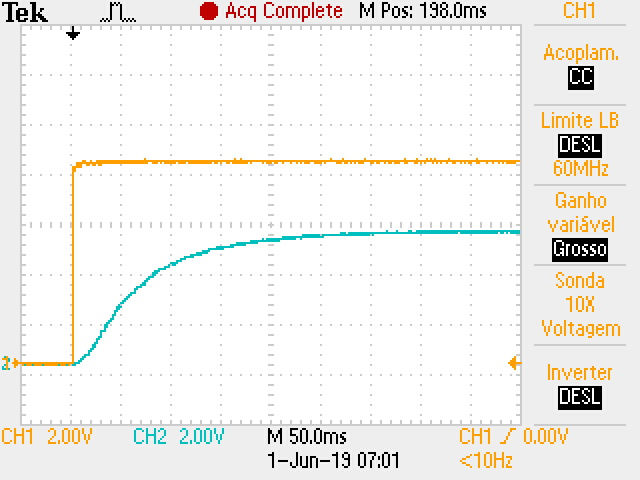
\includegraphics[height=10cm]{figuras/F0003TEK.JPG} % <- formatos PNG, JPG e PDF
\end{figure}
    
Obtivemos acesso a essas informações, captando a tela do osciloscópio através do botão print e salvando em um pendrive os arquivos gerados, contendo imagens da tela e um arquivo com os pontos do sistema, para mais tarde utilizarmos as informações dos pontos da curva do degrau e de sua resposta no MATLAB. 

Através do bloco de notas foram retirados os pontos anteriores ao instante de tempo zero e as vírgulas do arquivo gerado pelo osciloscópio, padronizando os arquivos para sua utilização. Na codificação do MATLAB, carregamos os dois arquivos já modificados com um plot, usando esse primeiro plot fizemos manualmente um deslocamento das leituras dos canais, observado a distância destes do ponto de origem, para que as duas leituras começassem nesse mesmo ponto, ambas foram deslocadas no eixo do tempo e apenas uma deslocada no eixo da amplitude corrigindo que no osciloscópio não era possível colocar as leituras perfeitamente no mesmo ponto. Também definimos em código o L, sendo este o tempo de atraso, ou tempo morto.

Logo após juntamos manualmente as duas curvas na origem, baseando-se no que já havia sido observado anteriormente, definimos também duas variáveis contendo os valores finais de leituras de entrada e saída do sistema, após isso calculamos o ganho K do sistema com base na relação dos dois valores finais, dividindo estas duas variáveis. Determinamos então qual seria o valor da amplitude de Tal, que consiste em 63,2\% do valor final da leitura de saída, sabendo o valor dessa amplitude achamos manualmente o valor de tempo Tal, buscando o ponto onde a curva de saída atinge o valor da amplitude.

Por fim foi determinada a função de transferência do sistema com base da fórmula (1/tal)/(s+(1/tal)) multiplicada pelo ganho K.
	
Com isto fizemos o projeto PI, achando o tempo de atraso e o tempo de subida utilizando o método da curva de reação, que consiste em colocar uma linha que tangenciasse a curva de resposta do degrau (figura 2), e seguindo o método de Ziegler e Nichols vistos em teoria, aplicamos as fórmulas do ganho proporcional (kp) e do ganho integrativo (ki).

\begin{figure}[H]
    \centering
    \caption{plot resposta degrau.}
    \label{fig:2}
    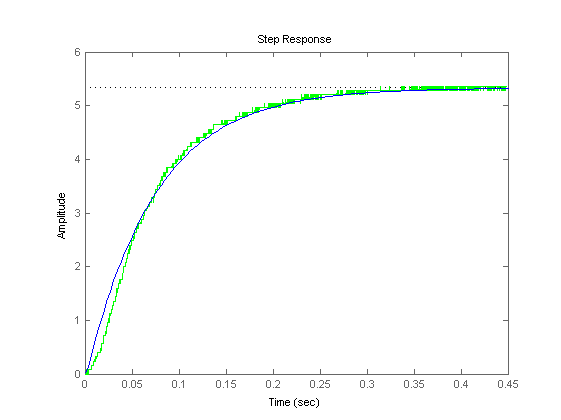
\includegraphics[height=10cm]{figuras/untitled.png} % <- formatos PNG, JPG e PDF
\end{figure}
	
Na figura 3 é mostrada as conexões utilizadas no projeto. Os cabos de alimentação positivos estavam ligados a placa, que transmitia para o gerador e o motor. Os cabos de alimentação negativos estavam ligados a todo o sistema, juntando CLP, fonte, gerador e motor. 
	
A placa de circuitos (figura 3) foi fornecida pelo professor-orientador para o experimento, ela possuía um botão que ao ser pressionado dividia a tensão fornecida ao motor, possibilitando simular as interferências na energia do sistema que possivelmente seriam analisadas em um projeto em nível industrial.

\begin{figure}[H]
	\centering
	\caption{Conexões.}
	\label{fig:3}	
	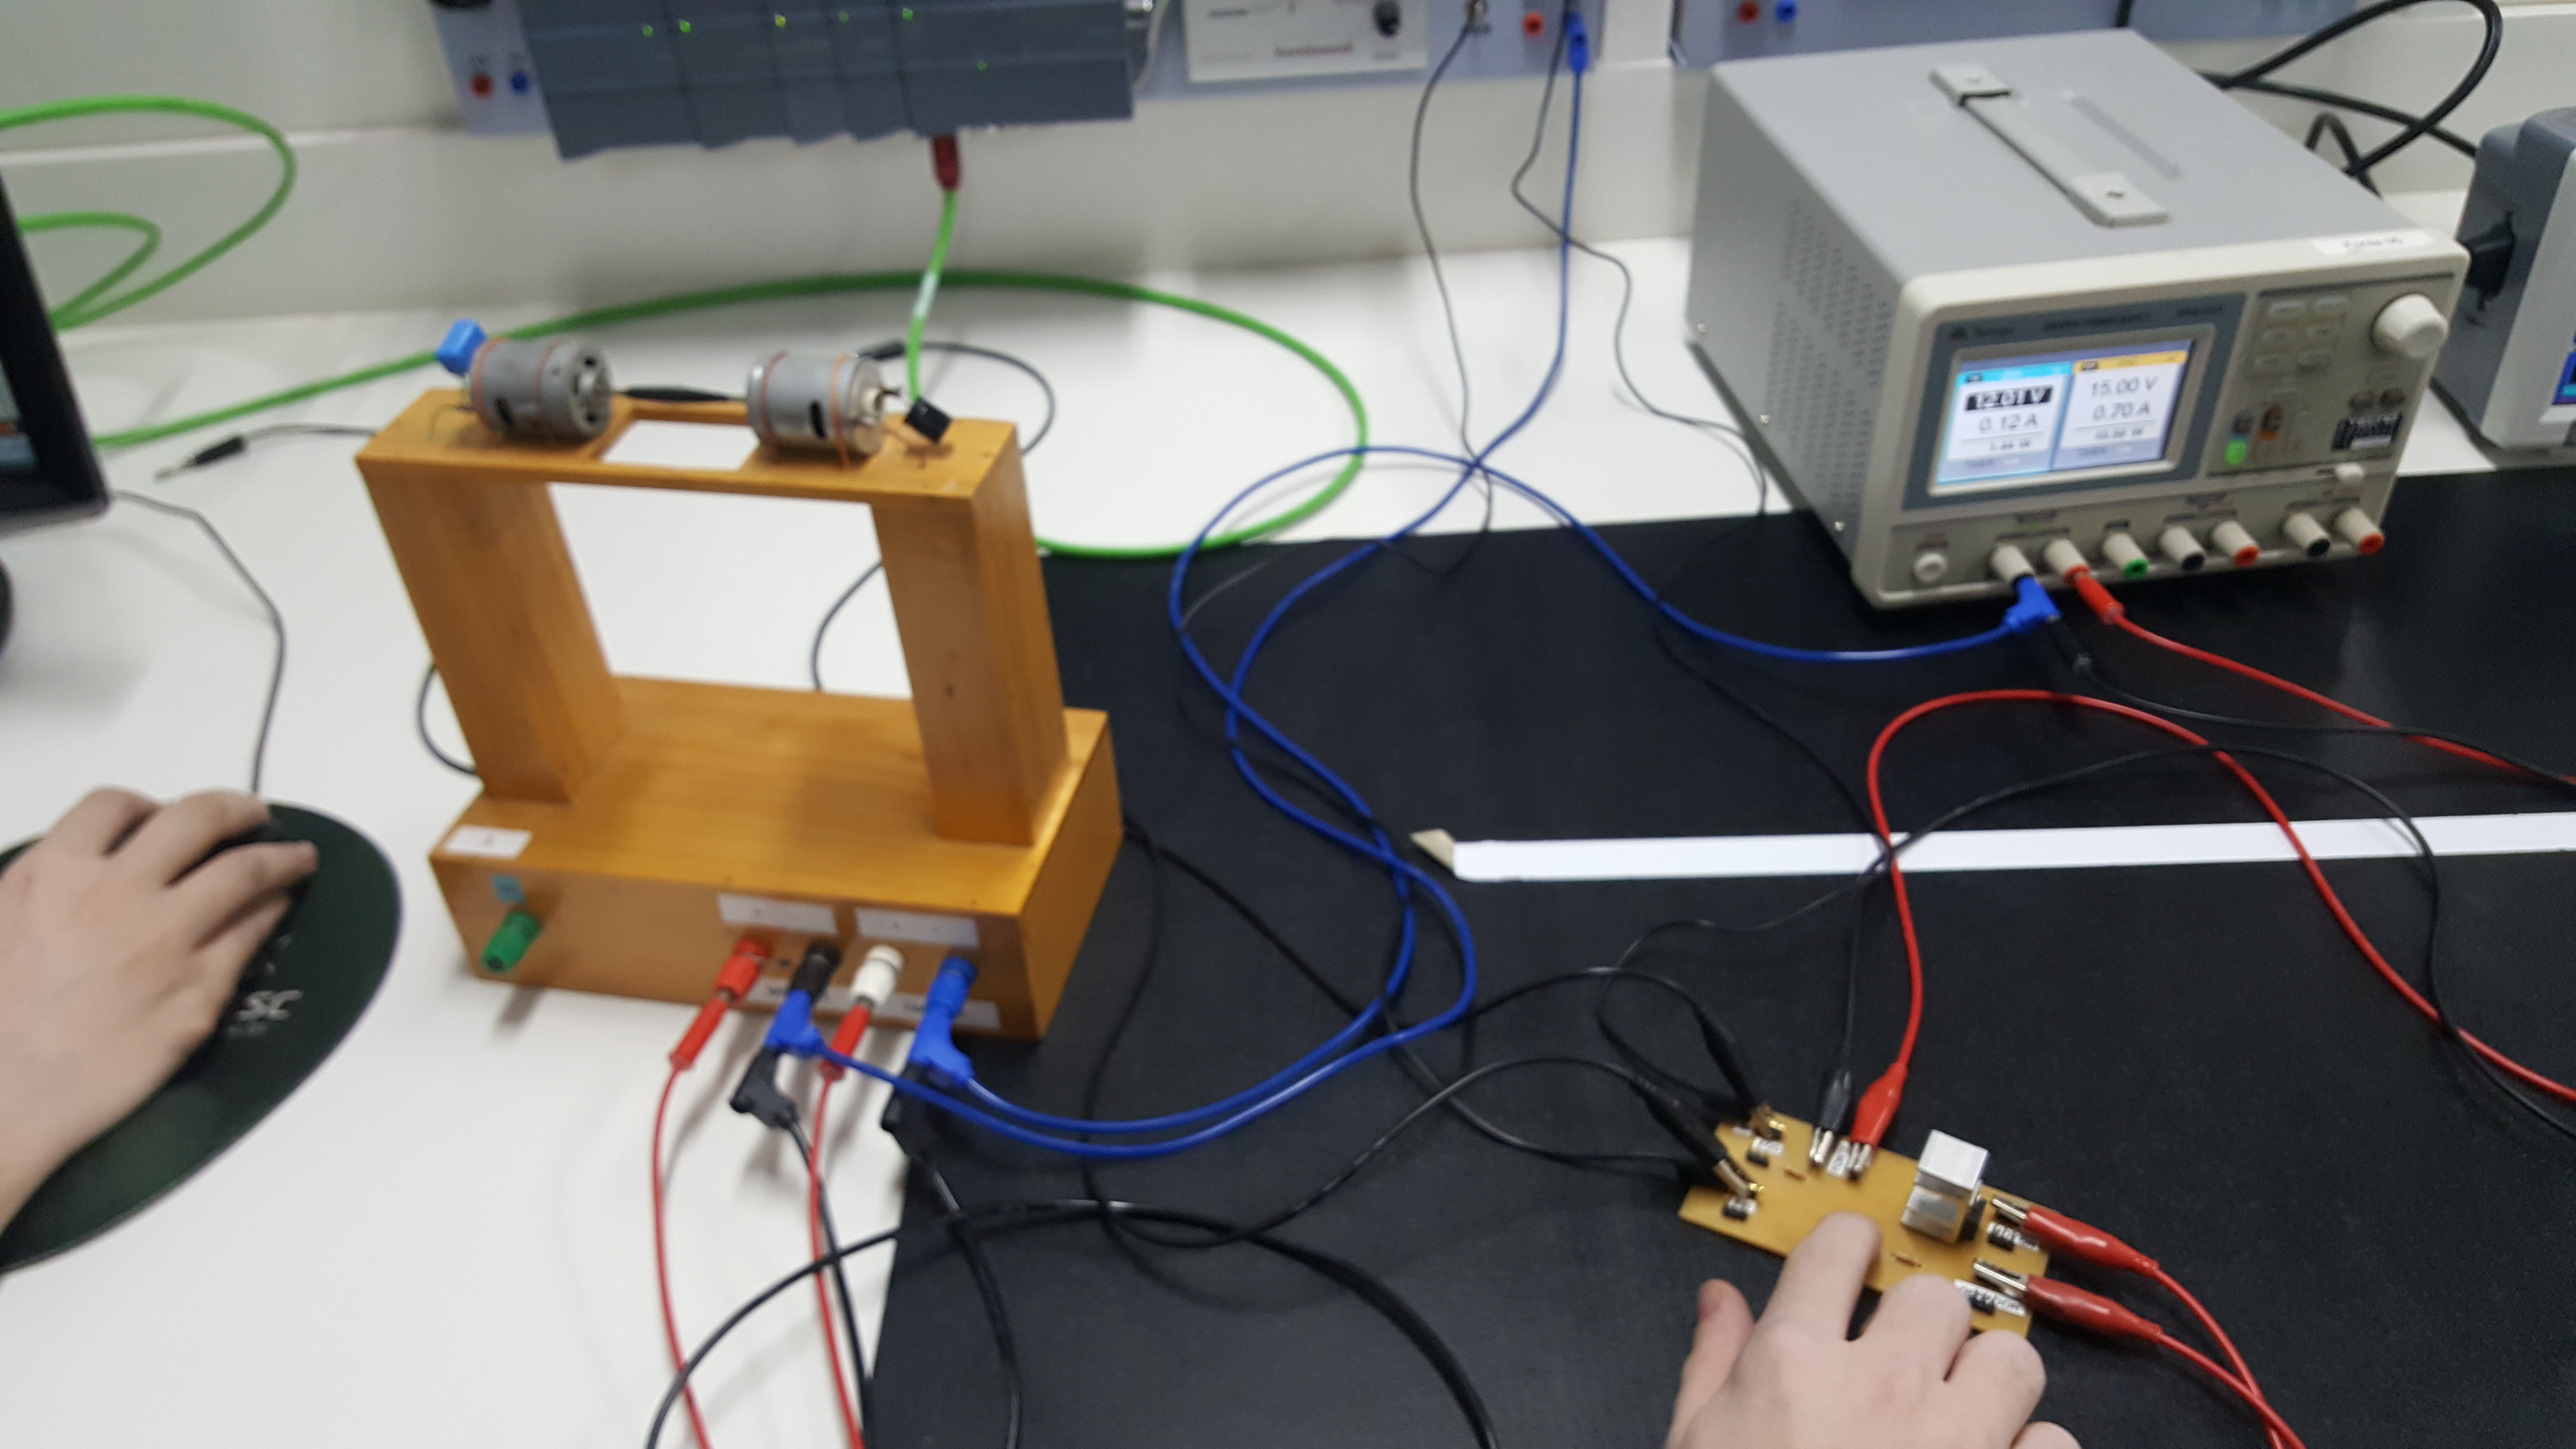
\includegraphics[height=8cm]{figuras/conexoes_bancada1.jpg} % <- formatos PNG, JPG e PDF
\end{figure}

Codificamos o CLP através do software TIAPortal para que ele recebesse e analisasse as informações de entrada e a partir disso retornasse a resposta adequada ao sistema. Para que o CLP processasse corretamente as informações tivemos que converter de inteiro para real (figura 4) para que então as informações pudessem ser inseridas no bloco PID do CLP (figura 5) e então convertemos novamente a saída, transformando de real para inteiro (figura 6), possibilitando que fosse enviada a resposta ao gerador.

\begin{figure}[H]
	\centering
	\caption{codificação CLP 1.}
	\label{fig:4}	
	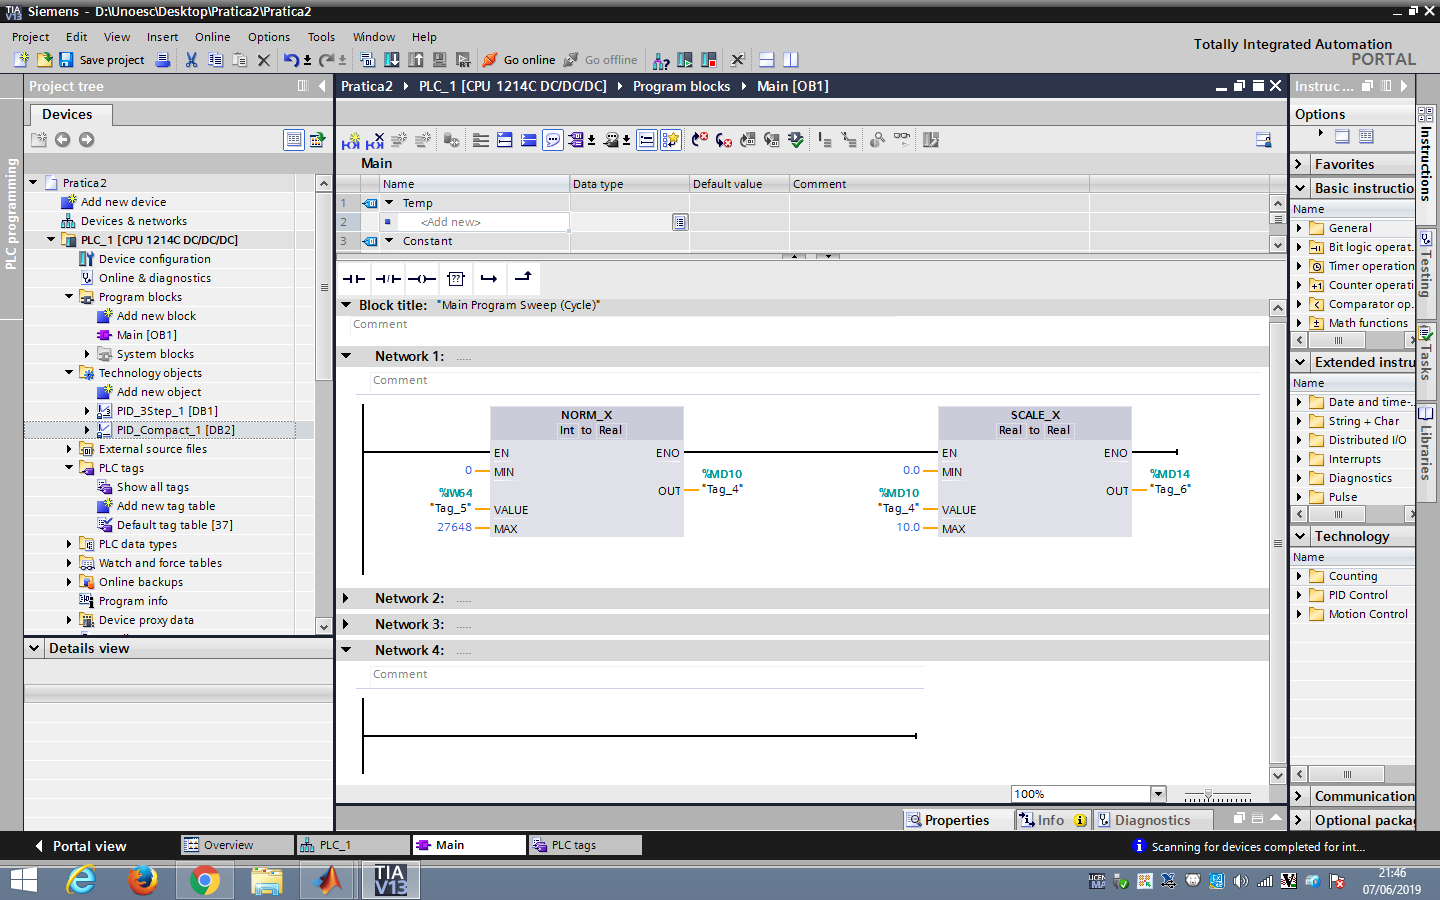
\includegraphics[height=10cm]{figuras/network1_clp.png} % <- formatos PNG, JPG e PDF
\end{figure}

\begin{figure}[H]
	\centering
	\caption{codificação CLP 2.}
	\label{fig:5}	
	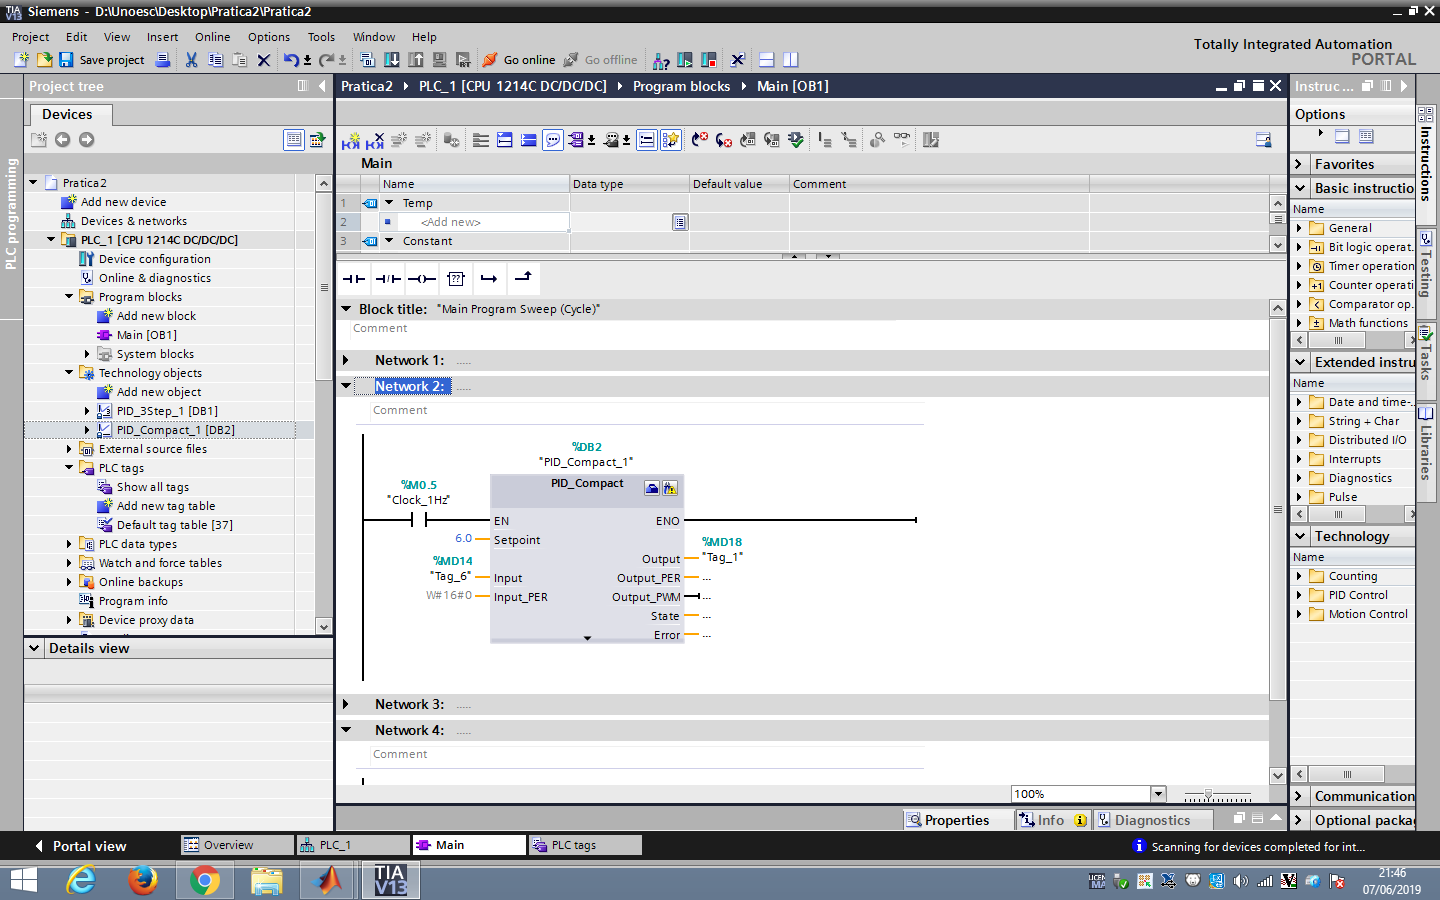
\includegraphics[height=10cm]{figuras/network2_clp.png} % <- formatos PNG, JPG e PDF
\end{figure}

\begin{figure}[H]
	\centering
	\caption{codificação CLP 3.}
	\label{fig:6}	
	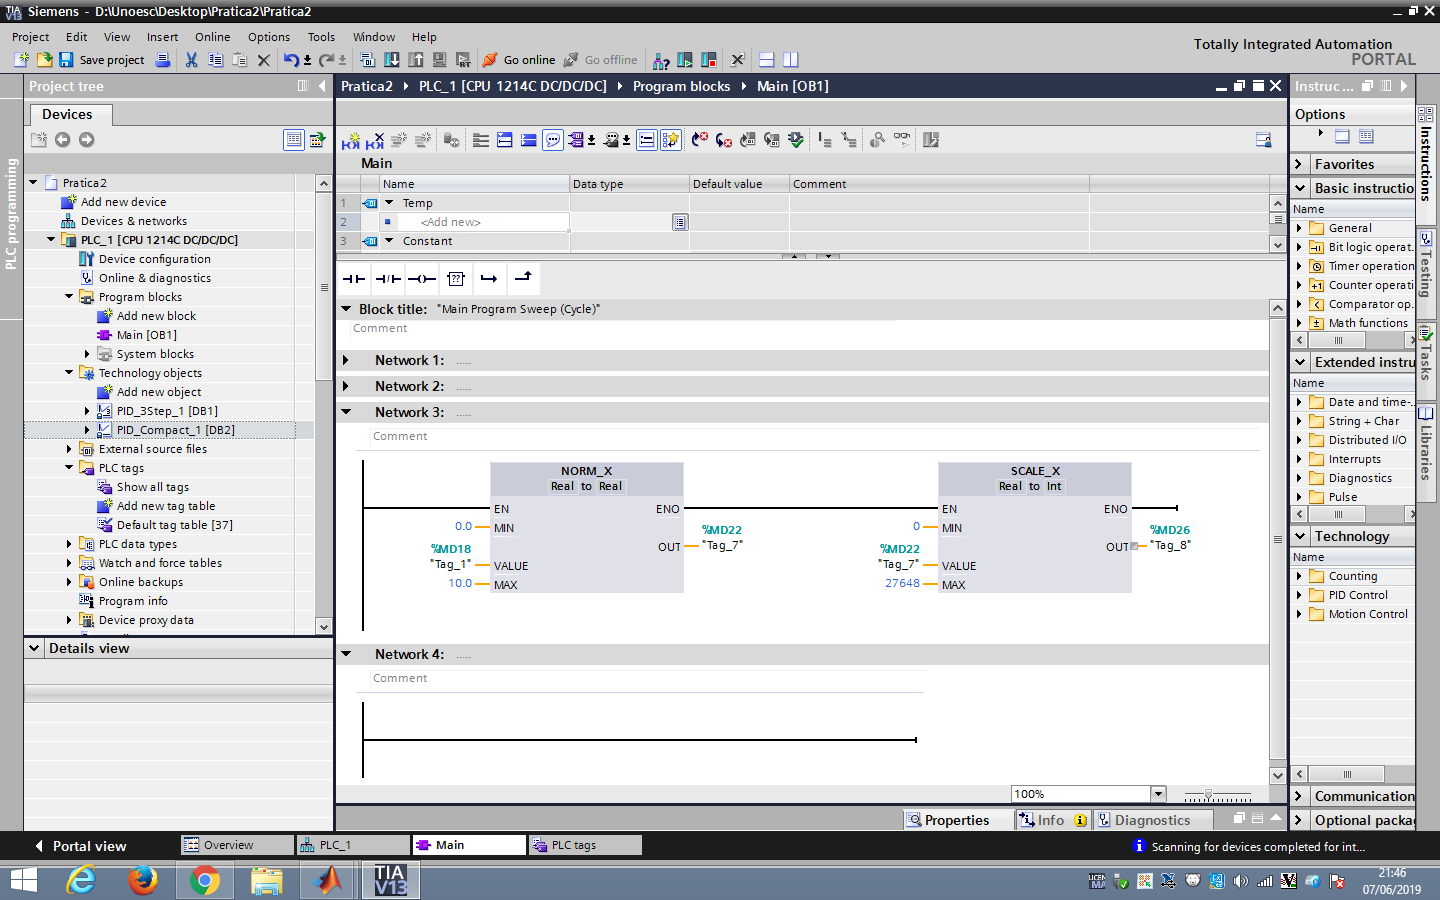
\includegraphics[height=10cm]{figuras/network3_clp.png} % <- formatos PNG, JPG e PDF
\end{figure}

Nas configurações do bloco PID, alteramos os parâmetros de input e output para que este funcionasse corretamente (figura 7), tivemos que alterar também os parâmetros do próprio PID (figura 8), pois sem os parâmetros adequados ele não retornava uma resposta satisfatória.

\begin{figure}[H]
	\centering
	\caption{Configuração bloco CLP 1.}
	\label{fig:7}	
	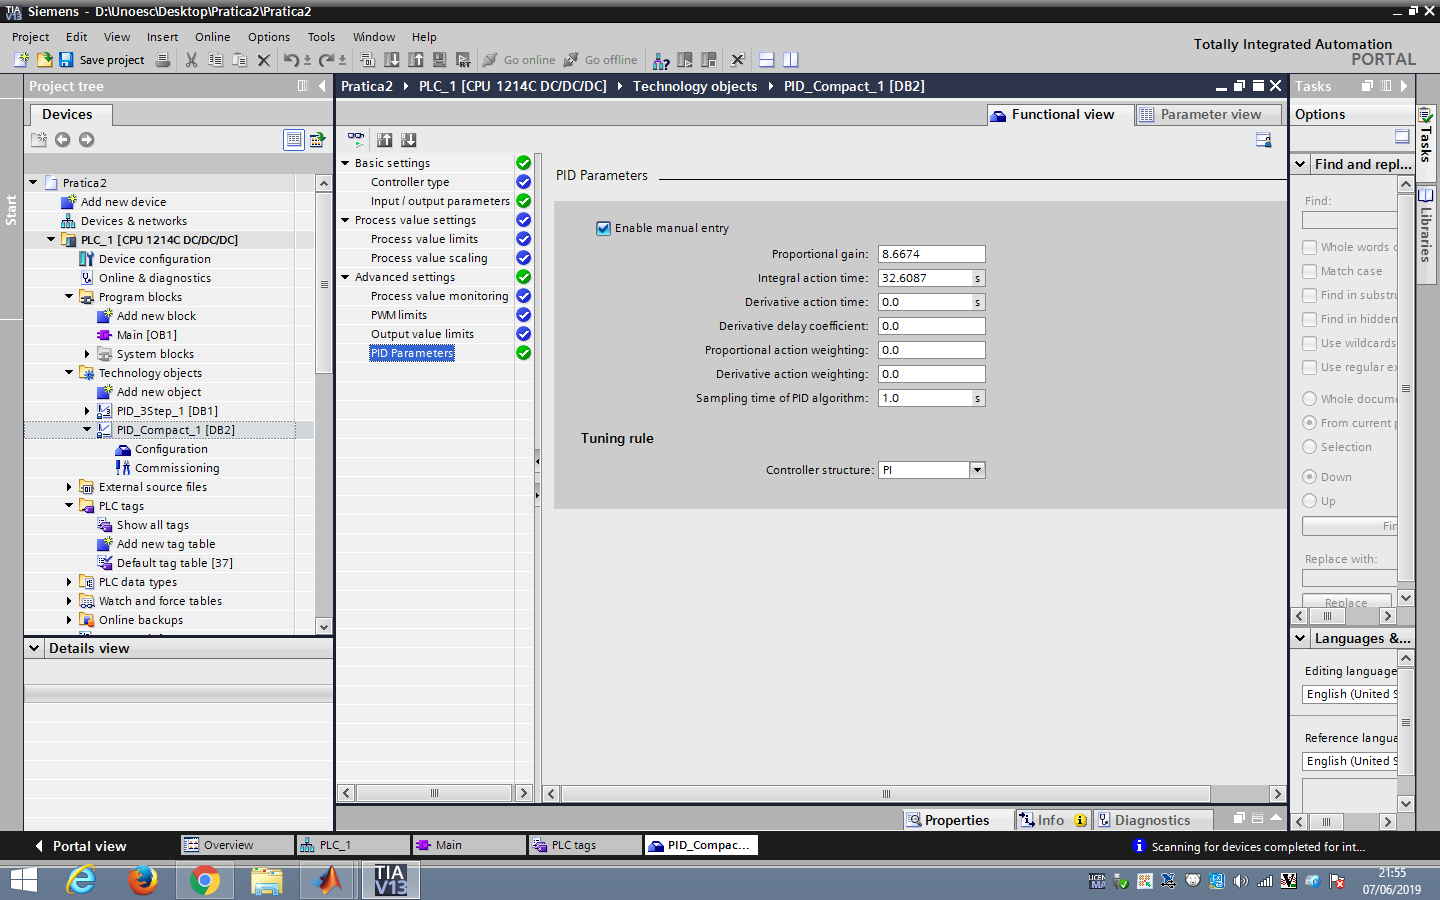
\includegraphics[height=10cm]{figuras/config_bloco_clp.png} % <- formatos PNG, JPG e PDF
\end{figure}

\begin{figure}[H]
	\centering
	\caption{Configuração bloco CLP 2.}
	\label{fig:8}	
	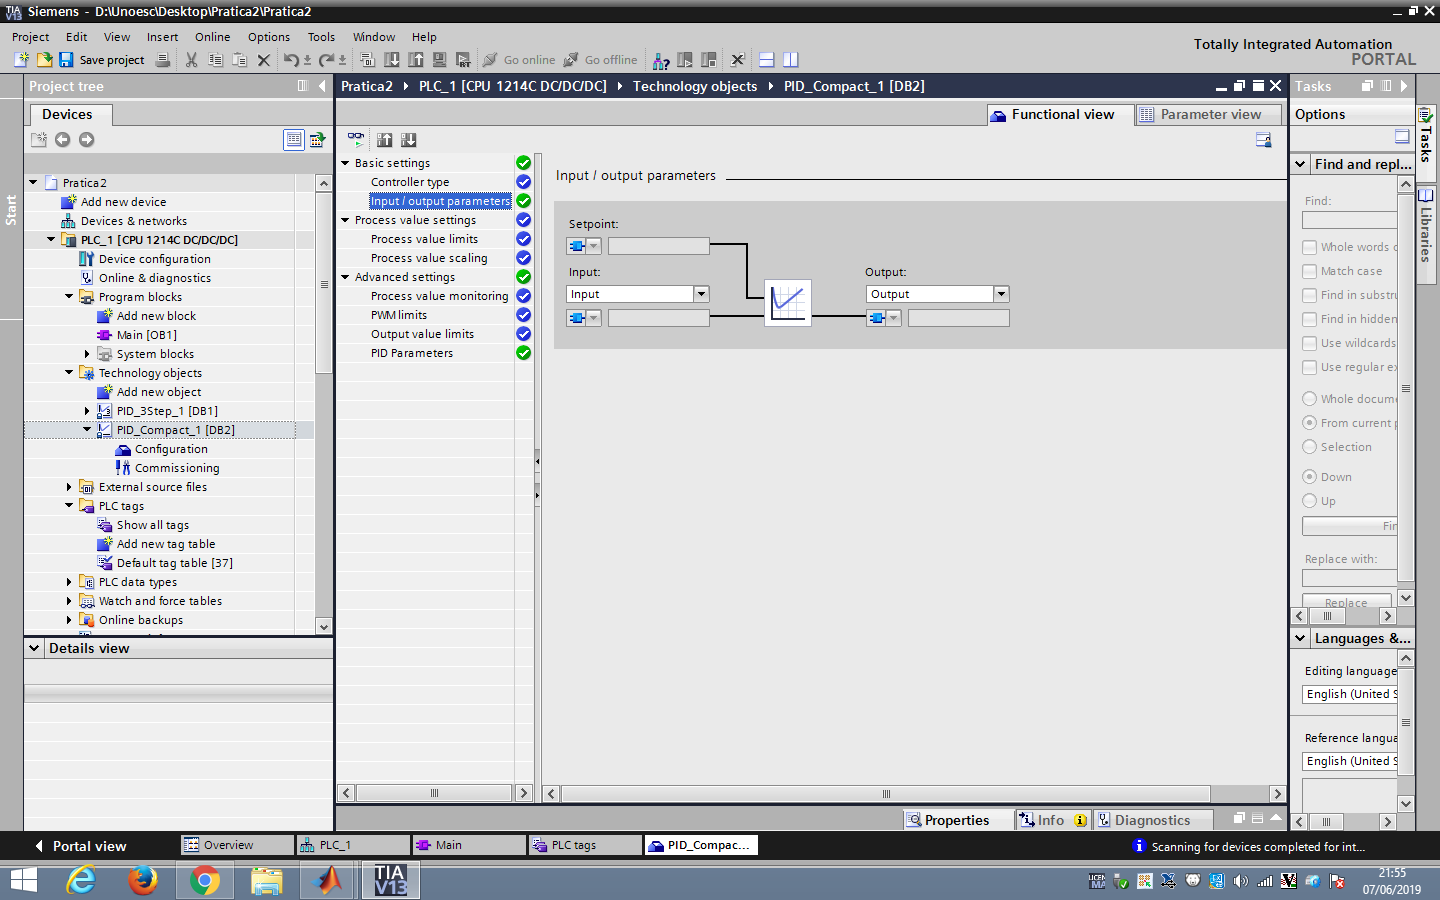
\includegraphics[height=10cm]{figuras/config_bloco_clp_2.png} % <- formatos PNG, JPG e PDF
\end{figure}

Por fim, tendo o sistema completo, pudemos observar as respostas de entrada e saída para cada interrupção causada pela divisão de tensão da placa (figura 9).

\begin{figure}[H]
	\centering
	\caption{Figura apenas inserida como exemplo.}
	\label{fig:9}	
	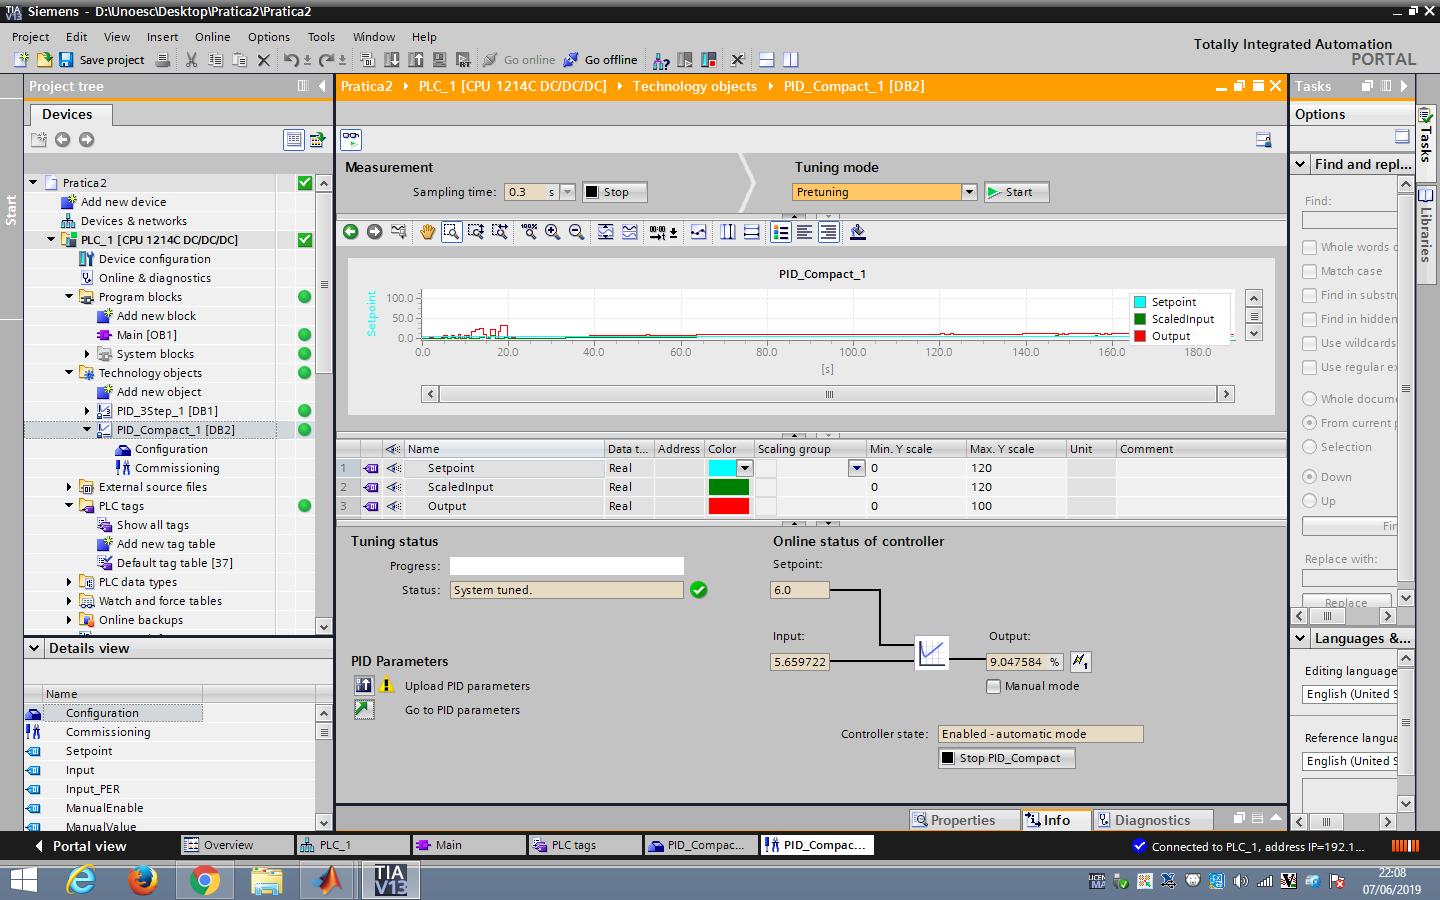
\includegraphics[height=10cm]{figuras/observacao.png} % <- formatos PNG, JPG e PDF
\end{figure}

\section{Conclusão}

Sistemas de controle são complexos, diversas são as dificuldades encontradas na prática que outrora jamais seriam vistas apenas em teoria. Este projeto possibilitou aos acadêmicos um vislumbre prático de uma aplicação de sistema de controle, entendimento da teoria vista em aula e das dificuldades de criação e adaptação do projeto. Durante o projeto, lidamos com algumas dificuldades de implementação, como por exemplo os valores calculados no Matlab que não atenderam as necessidades, tivemos que fazer algumas alterações manuais e recalcular os valores para que o sistema funcionasse corretamente. A resposta do sistema após as alterações foi muito satisfatória, pudemos ver o sistema implementado e funcionando, onde a cada interrupção o CLP compensava a saída para que esta permanecesse estável e sem oscilações.

\begin{thebibliography}{1}
\bibitem{hist}
Museu das Telecomunicações. História das telecomunicações, [2001].
\emph{DORF, Richard C.; BISHOP, Robert H. Sistemas de controle modernos. 8. ed. Rio de Janeiro: LTC, 2001. 661 p. ISBN 0201208649.}

\end{thebibliography}

\pagebreak
\clearpage
\newpage
\end{document}
